\subsection{HWP $I\rightarrow P$}
\label{IP downstream of HWP}
\paragraph{Description:}
When passing through the HWP, incoming polarized radiation is rotated by $2\chi$, where $\chi$ is the rotation angle of the HWP optical axis. The signal is finally seen by the detectors at $4\chi$. Any unpolarized signal which is modulated at $4\chi$ represents a source of systematics. A list of possible sources of spurious $4\chi$ signals can be found in Sec.III of~\cite{ABS}. The main source comes from non-normal incidence, since the reflected signal by the crystal itself and the AR coating is partly polarised and thus modulated by $4\chi$. Other sources include polarized emission due to differential transmission and differential absorption. Although these emission is usually modulated at $2\chi$, it might be further modulated at $4\chi$ due to HWP misalignment and/or non uniform AR coating.

\paragraph{Plan to model and/or measure:}
We expect the $I\rightarrow P$ leakage to be small. Nevertheless, it needs to be carefully modelled and understood, as the major unpolarised sources (emissivity from warm optical elements in the optical chain, atmospheric noise and unpolarised CMB) are many order of magnitudes higher than the actual signal of interest, the CMB polarization signal. For these reasones, the SRF is 4.

In order to model this effect, we need the global unpolarized power incident on the sky-side of the HWP, the HWP physical properties as well as the proprties of any AR coating, and a mapping between the incidence angle of the incoming radiation and the position on focal plane where the incoming radiation is going to be collected. 

We model the incoming and outgoing signals, the HWP and the detectors following the Mueller matrix approach. We make use of the transfer matrix formalism to model the Mueller matrix for the HWP and AR coating stack~\cite{Tom_TM}. In the case of the SAC, the incoming radiation can be represented as a plane wave. Therefore, at each incidence angle roughly corresponds a specific position on the focal plane where the signal is focused and collected. The mapping between the incidence angle and the position on the focal plane should be accurately modelled through ray-tracing techniques. However, a first estimate can be obtained by assuming a simple relation, such as 
\begin{equation}\label{eq:fp}
\delta x= f \delta \theta,
\end{equation}
where $\delta x$ is the distance on the focal plane with respect to the central pixel, $\delta \theta$ is the angular distance with respect to normal incidence, and $f$ represents the scaling coefficient between $\theta$ and $x$ (a good approximation for $f$ is $f\simeq 1\,\mathrm{cm\,deg^{-1}}$).

To predict the magnitude of the effect, we assume that unpolarised signal passes through the HWP at a generic incidence angle $\theta$. We compute the output signal as a function of the rotation angle $\chi$ of the HWP. We fit this signal with a harmonic series of cosine terms and isolate the coefficient $A_4$ of the $4\chi$ component. This represents our estimate of $I\rightarrow P$ leakage. This calcuation is done for different incidence angles $\theta$. The set of $A_4$ coefficients as a function of $\theta$ is then assigned a position on the focal plane according to Eq.~\ref{eq:fp}.

\paragraph{Uncertainty/Range:}
An example of $I\rightarrow P$ leakage estimated following the approach above is shown in Fig.~\ref{fig:ip_fp}. The figure shows the normalized $A_4$ component as collected on the focal plane, coming from an incoming unpolarized radiation which passes through the HWP. The HWP is achromatic and optimized to cover both the $90\,\mathrm{GHz}$ and $150\,\mathrm{GHz}$ bands. As expected, the $I\rightarrow P$ leakage is small, lower than 0.02\%. As also expected, the higher contribution is relegated to the edges of the focal plane, as it comes from the largest incidence angles $\theta\sim 20^\circ$.

\begin{figure}
\begin{center}
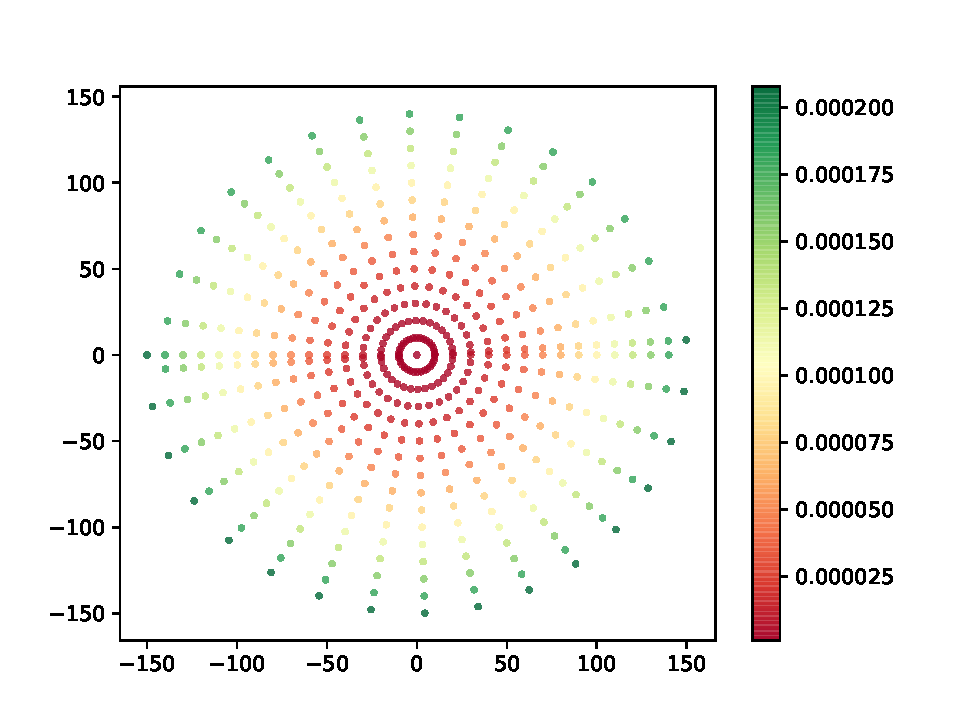
\includegraphics{figures/A4_focalPlane.pdf}
\end{center}
\caption{Normalized $A_4$ component as collected on the focal plane, coming from an incoming unpolarized radiation which passes through the HWP. The incidence angles are in the range $[-20^\circ,20^\circ]$. The relation between the incidence angle and the position on the focal plane is given in Eq.~\ref{eq:fp}. The HWP is achromatic and optimized to cover both the $90\,\mathrm{GHz}$ and $150\,\mathrm{GHz}$ bands. The assumed thickness and indexes of the sapphire are the same as in Tab.2 of~\cite{PB2a_WHWP}.}\label{fig:ip_fp}
\end{figure}

\paragraph{Parameterization:}
The $I\rightarrow P$ leakage can be parametrized as the coefficient of the 4-th harmonic in the series expansion used to parametrize the output signal as transmitted by the HWP. This coefficient can be estimated as a function of the incidence angle and then assigned to a position on the focal plane. This last assignment requires ray-tracing techniques and therefore knowledge of the optical chain. However, a quick estimate can be done by assuming a simple relation between incidence angle and position on the focal plane, especially in the case of SAC.
